\chapter{Integer Programming}
\todo[inline]{8 pages: \cancel{||||}~|}

\todo[inline]{glue text}

\begin{definition}[(Linear) \gls{IP}]
  An \gls{IP} is a system of integer variables
  \(x \in \gls{Z}^n\) with a set of constraints on them and often an 
  objective function \(c^T x\). We consider only the case where the 
  constraints are linear: \(Ax \leq b\) or \(Ax \geq b\).
\end{definition}

\todo[inline]{glue text}

\begin{problem}[\gls{IP} in canonical form \cite{combinatorial_optimization}]
  \begin{alignat*}{2}
    &\text{maximize } & c^Tx \\
    &\text{subject to } & Ax &\leq b \\
    && x &\geq 0 \\
    && x &\in \gls{Z}
  \intertext{or}
    &\text{minimize } & c^Tx \\
    &\text{subject to } & Ax &\geq b \\
    && x &\leq 0 \\
    && x &\in \gls{Z}
  \end{alignat*}
\end{problem}

\begin{theorem}
  Solving \gls{IP}[s] is NP-hard.
\end{theorem}

\begin{proof}
  Even the special case where there is no objective function, only
  binary variables, and only equality constraints is NP-complete
  \cite{karp_np_complete}. Therefore the more general problem is
  NP-hard.
\end{proof}

% \section{SAT}
% \todo[inline]{glue text}
% 
% \begin{definition}[SAT]
%   \ldots\todo[inline]{definition}
% \end{definition}
% \todo[inline]{glue text}
% 
% \begin{problem}[IP formulation of SAT]
%   \ldots\todo[inline]{problem}
% \end{problem}

\section{Vertex Cover}
\todo[inline]{glue text}

\begin{definition}[Vertex Cover]
  \label{def:vertex_cover}
  Given an undirected graph \(G=(V,E)\), a vertex cover
  \(\gls{VC} \subseteq V\) for \(G\) is a vertex set such that
  every edge \(e \in E\) is incident to at least one vertex
  \(v \in \gls{VC}\):
  \[ \forall e \in E: \exists v \in \gls{VC}: v \in e \]
\end{definition}

\todo[inline]{glue text}

\begin{definition}[Minimal Vertex Cover]
  A vertex cover \gls{VC} for an undirected graph
  \(G=(V,E)\) is minimal if there is no vertex
  \(v \in \gls{VC}\) such that
  \(\gls{VC} \setminus \{v\}\) remains a vertex cover.
\end{definition}

\todo[inline]{glue text}

\begin{definition}[Minimum Vertex Cover]
  A vertex cover \gls{VC} for an undirected graph
  \(G=(V,E)\) is minimum if there is no other vertex cover
  \(\gls{VC}[']\) for \(G\) which has fewer vertices:
  \[
    \forall~V_{\text{cover}}'\text{ vertex cover} :
    |\gls{VC}| \leq |\gls{VC}[']|
  \]
\end{definition}

\begin{figure}[ht]
  \centering
  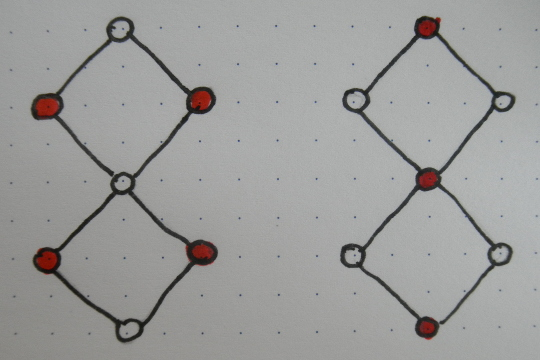
\includegraphics[width=0.5\textwidth]{img/example_vertex_cover.jpg}
  \todo[inline]{replace}
  \caption{\label{fig:example_vertex_cover}Example of minimal vs. minimum vertex cover}
\end{figure}

\todo[inline]{glue text}

\begin{problem}[\gls{IP} Formulation of Minimum Vertex Cover]
  \begin{alignat*}{3}
    &\text{minimize } & \sum\limits_{v \in V} x_v \\
    &\text{subject to } & \forall \{v,w\} \in E : &~& x_v + x_w &\geq 1 \\
    && \forall v \in V : &~& x_v &\in \{0,1\}
  \end{alignat*}
\end{problem}

\todo[inline]{glue text}

\begin{theorem}
  Vertex Cover is NP-complete. \cite{karp_np_complete}
\end{theorem}

\todo[inline]{glue text}

\begin{definition}[\Gls{wcover} Graph]
  \label{def:well_covered}
  An undirected graph \(G=(V,E)\) is \gls{wcover} iff every minimal
  vertex cover for \(G\) is also a minimum vertex cover for \(G\).
  \cite{graph_well_covered}
\end{definition}

\todo[inline]{glue text}

\begin{theorem}
  \label{thm:well_covered_vertex_cover}
  In a \gls{wcover} graph, all minimal vertex covers have the same
  cardinality. \cite{graph_well_covered}
\end{theorem}

\section{Independent Set}

\todo[inline]{glue text}

\begin{definition}[Independent Set]
  \label{def:independent_set}
  Given an undirected graph \(G=(V,E)\), an independent set
  \(\gls{IS} \subseteq V\) is a vertex set such that no two
  vertices \(v,w \in \gls{IS}\) are incident to the same edge 
  \(\{v,w\} \in E\):
  \[
    \forall v \in \gls{IS}:
    \forall \{v,w\} \in E:
    w \not\in \gls{IS}
  \]
\end{definition}

\todo[inline]{glue text}

\begin{definition}[Maximal/Maximum Independent Set]
  \label{def:max_independent_set}
  For an undirected graph \(G=(V,E)\), an independent set
  \(\gls{IS}\subseteq V\) is maximal if there is no vertex
  \(v \in V\setminus \gls{IS}\) such that
  \(\gls{IS} \cup \{v\}\) remains an independent set. It is
  maximum if there is no independent set \(\gls{IS}'\) with
  larger cardinality.
\end{definition}

\todo[inline]{glue text}

\begin{problem}[\gls{IP} Formulation of Maximum Independent Set]
  \begin{alignat*}{3}
    &\text{maximize } & \sum\limits_{v \in V} x_v \\
    &\text{subject to } & \forall \{v,w\} \in E : &~& x_v + x_w &\leq 1 \\
    && \forall v \in V : &~& x_v &\in \{0,1\}
  \end{alignat*}
\end{problem}

\todo[inline]{glue text}

\begin{theorem}[Independent Set and Vertex Cover]
  \label{thm:independent_set_vertex_cover}
  For an undirected graph \(G=(V,E)\), \(\gls{IS} \subseteq V\)
  is a maximum independent set iff
  \(\gls{VC} = V \setminus \gls{IS}\) is a minimum vertex
  cover.
\end{theorem}

\begin{proof}
  Let \gls{VC} be a vertex cover for \(G\). 
  \begin{alignat*}{1}
    \forall e \in E : \exists v \in \gls{VC} : v \in e
    &\iff \forall \{v,w\} \in E :
      v \in \gls{VC} \lor w \in \gls{VC} \\
    &\iff \forall \{v, w\} \in E :
      \lnot(v \not\in \gls{VC} \land w \not\in \gls{VC}) \\
    &\iff \forall \{v, w\} \in E :
      \lnot(v \in (V \setminus \gls{VC})
        \land w \in (V \setminus \gls{VC})) \\
    &\iff \forall v \in (V \setminus \gls{VC}) :
      \forall \{v, w\} \in E :
      w \not\in (V \setminus \gls{VC}) \\
    &\iff (V \setminus \gls{VC}) \text{ independent set}
  \end{alignat*}
  
  Assume \gls{VC} is a minimum vertex cover for \(G\) and the
  independent set \(\gls{IS} = V \setminus \gls{VC}\) is not maximum.
  Then there is an independent \(\gls{IS}['] \subseteq V\) with
  \(|\gls{IS}| < |\gls{IS}[']|\). But then for the vertex cover
  \(\gls{VC}['] = V \setminus \gls{IS}[']\) the following holds:
  \(|\gls{VC}[']| < |\gls{VC}|\)---which is a contradiction to
  \gls{VC} being minimum. The same argumentation applies in the other
  direction.
\end{proof}

\todo[inline]{glue text}

\begin{theorem}[Independent Set in \gls{wcover} Graphs]
  \label{thm:well_covered_independent_set}
  For a \gls{wcover} graph \(G=(V,E)\), every maximal independent set
  has the same size and is therefore maximum.
\end{theorem}

\begin{proof}
  \Cref{thm:well_covered_independent_set} follows directly from
  \cref{%
    def:well_covered,%
    thm:well_covered_vertex_cover,%
    thm:independent_set_vertex_cover%
  }.
\end{proof}

\todo[inline]{examples: \cref{fig:example_vertex_cover}}

\todo[inline]{glue text}

\begin{algorithm}
  \DontPrintSemicolon
  
  \KwIn{Undirected graph \(G=(V,E)\)}
  \KwOut{Maximal independent set \(\gls{IS} \subseteq V\) for \(G\)}
  
  Set \(\gls{IS} = \emptyset\) \;
  \ForEach{\(v \in V\)}{
    \If{\(\forall \{v,w\} \in E: (w \not\in \gls{IS})\)}{
        Set \(\gls{IS} = \gls{IS} \cup \{v\}\) \;
    }
  }
  \KwRet{\gls{IS}}
  \caption{\label{alg:greedy_independent_set}Greedy algorithm for independent set}
\end{algorithm}

\todo[inline]{glue text}

\begin{theorem}[Correctness and Complexity of \Cref{alg:greedy_independent_set}]
  \label{thm:greedy_independent_set}
  \Cref{alg:greedy_independent_set} always finds a maximal independent
  set in \(O(|E|)\) time.
\end{theorem}

\begin{proof}
  Because the vertices are processed sequentially, for every edge
  \(\{v,w\} \in E\) at most one of \(v\) and \(w\) is added to
  \gls{IS}. Therefore \gls{IS} is an independent set. Additionally 
  every vertex \(v \in V\) is processed and if there is no
  \(w \in \gls{IS}\) with \(\{v,w\} \in E\) then \(v \in \gls{IS}\).
  So \gls{IS} is maximal.
  
  The for-loop runs \(|V|\) times but the if-statement is only
  executed twice for every edge \(e \in E\). Every other statement
  runs in \(O(1)\) time. Thus \cref{alg:greedy_independent_set} needs
  \(O(|E|)\) time.
\end{proof}

\todo[inline]{glue text}

\begin{theorem}[\Cref{alg:greedy_independent_set} in \gls{wcover} Graphs]
  \label{thm:well_covered_maximum_independent_set}
  For a \gls{wcover} graph \cref{alg:greedy_independent_set} always
  finds a maximum independent set in \(O(|E|)\) time.
\end{theorem}

\begin{proof}
  \Cref{thm:well_covered_maximum_independent_set} follows directly
  from \cref{thm:well_covered_independent_set,thm:greedy_independent_set}.
\end{proof}

\section{Set Cover}
\ldots\todo[inline]{evaluate if we really need set cover}

% In the next recess Greg and his friends were discussing again what
% to play. It was always hard to find games that everybody liked.
% For example, Greg likes to play tables tennis or Duck, Duck, Goose but
% does not want to play soccer. Suddenly Greg had an idea: What about
% making a list of everybody's first and second choice and then 
% finding groups which could play together. His friends agree and
% you can see the result in \cref{tab:game_voting}.
% 
% \begin{table}[ht]
%   \centering
%   \begin{tabular}{l|cccc}
%     & table tennis & Duck, Duck, Goose & soccer & swings \\
%     \hline
%     Greg  & 1 &   &   & 2 \\
%     Joey  & 2 & 1 &   &   \\
%     Susan & 1 &   & 2 &   \\
%     Bella &   &   & 2 & 1 \\
%     Jenny & 1 & 2 &   &   \\
%     Jason &   &   & 1 & 2 \\
%     Alice &   & 2 &   & 1 \\
%     Bob   &   & 1 & 2 &   \\
%   \end{tabular}
%   \caption{\label{tab:game_voting}Voting of Greg and his friends}
% \end{table}

% Then Greg went to Mrs. Lloyd and asked her how they could find the 
% best solution. Firstly, she made another list
% (\cref{tab:example_set_cover}) where she put all the children's
% names for each game and summed up their preferences.%
% \footnote{Note that I cheated here: Usually you would divide the
% sum of preferences by the number of children who want to play the
% game. But Greg did not know yet how to divide, so I made all the
% groups have equal size.}

% \begin{table}[ht]
%   \centering
%   \begin{tabular}{lc}
%     table tennis (Greg, Joey, Susan, Jenny): & 4 \\
%     Duck, Duck, Goose (Joey, Jenny, Alice, Bob): & 6 \\
%     soccer (Susan, Bella, Jason, Bob):       & 7 \\
%     swings (Greg, Bella, Jason, Alice):      & 6 \\
%   \end{tabular}
%   \caption{\label{tab:example_set_cover}Summed up preferences for each game}
% \end{table}

% Mrs. Lloyd showed the children that there were no two games to cover
% all of them --- so they needed to split up into at least three groups.
% The best way to do so was to play table tennis, Duck, Duck, Goose, and
% on the swings. That was everybody's first choice besides for Jason.
% The problem Mrs. Lloyd solved is an instance of the minimum weight 
% set cover problem.

\begin{problem}[Minimum Weight Set Cover]\label{prob:mwsc}
  \hfill
  \begin{labeling}{\hspace{4em}}
    \item[\textbf{Given:}]
      A ``universe'' (set) of objects \(U\), 
      subsets \(S = \{S_i\}\)
      such that \(\bigcup\limits_{S_i \in S} S_i = U\),
      and a weight function \(c : S \to \gls{R}_+\)
    \item[\textbf{Sought:}]
      A set \(R \subseteq S\)
      which covers the universe, i.e. 
      \(\bigcup\limits_{S_i \in R} S_i = U\)
      and minimizes \(\sum\limits_{S_i \in R} c(S_i)\)
  \end{labeling}
\end{problem}

\Cref{prob:mwsc} is NP-hard \cite{set_cover} and the related decision 
problem was already one of the problems Karp has shown to be 
NP-complete \cite{karp_np_complete}.

%---------------------------------------------------------------------##########
